\subsection{Закон сохранения энергии и типы орбит}
Для движения тела c массой $m$ в гравитационном  в поле тела 
с массой \linebreak $M\gg m$ со скорость $v$ на расстоянии $r$ от 
гравитационного центра справедливо следующее соотношение: 
\begin{equation}
\frac{m v^2}{2}-\frac{GM m }{r}=E_0,
\end{equation}
где $E_0$ --- постоянная величина, если на тело не действуют
внешние силы кроме силы притяжения к центральному телу, 
равная сумме кинетической и потенциальной энергии тела.

Если $E_0>0$, то траектория тела --- {\itshape гипербола}, 
ветви которой асимптотически приближаются к двум прямым.

Если $E_0=0$, то траектория тела --- {\itshape парабола}. При 
параболической и гиперболический траекториях движение не 
ограничено (инфинитно).

Если $E_0<0$, то траектория тела --- {\itshape эллипс}. При 
эллиптической траектории движение ограничено (финитно).

Параболическая скорость --- минимальная, при которой 
тело покидает центральное тело. Она также называется
{\itshape вторая космическая скорость}. Выражение для нее 
имеет следующий вид:\begin{equation}
v_{2}=\sqrt{\frac{2GM}{r}}
\end{equation}

На Рис. \ref{pic:orbits} представлены примеры возможных траекторий тела 
относительно центрального (точка C). При $v_0 > v_{2}$ --- тело движется 
по гиперболе, при $v_0 = v_{2}$ --- по параболе, 
а при $v_0 < v_{2}$ --- по эллипсу.
\begin{figure}[h!]
\centering
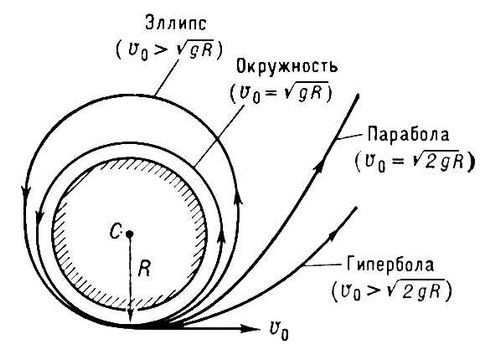
\includegraphics[width = 0.5\textwidth]{Space-speed}
\caption{Возможные траектории тела \label{pic:orbits}}
\end{figure}

\textit{Первая космическая скорость} --- минимальная скорость, необходимая для того, чтобы маломассивное тело стало искусственным спутником центрального тела.
\begin{equation}v_1=\sqrt{\frac{GM}{R}}
\end{equation}
Где $M$ --- масса массивного тела.

\textit{Вторая космическая скорость} --- минимальная скорость, необходимая для того, чтобы маломассивное тело преодолело гравитационное притяжение центрального тела и покинуло замкнутую орбиту вокруг последнего. 
\begin{equation}v_2=v_p=\sqrt{2gR}=\sqrt{\frac{2GM}{R}}=\sqrt{2}v_1
\end{equation}

$v_1$ и $v_2$ на некоторых телах Солнечной системы:
\begin{table}[h!]
\centering
\begin{tabular}{|c|c|c|}
\hline
\textbf{Планета} & $\mathbf{v_1}$,\textbf{км/c} & $\mathbf{v_2}$,\textbf{км/c}\\
\hline
Солнце & 436,8 & 617,7\\
\hline
Меркурий & 3,0 & 4,3\\
\hline
Венера & 7,4 & 10,5\\
\hline
Земля & 7,9 & 11,2\\
\hline
Луна & 1,7 & 2,4\\
\hline
Марс & 3,5 & 5,0\\
\hline
Юпитер & 42,0 & 59,5\\
\hline
Сатурн & 25,1 & 35,5\\
\hline
Уран & 15,0 & 21,3\\
\hline
Нептун & 16,6 & 23,5\\
\hline
\caption{$v_1$ и $v_2$ на некоторых телах Солнечной системы}
\end{tabular}
\end{table}

Скорость искусственного небесного тела на высоте $h$.\begin{equation}v_h=\sqrt{\frac{GМ}{R+h}}=\sqrt{\frac{gR^2}{R+h}}
\end{equation}

\textit{Третья космическая скорость} --- минимальная скорость, которую необходимо придать находящемуся вблизи поверхности Земли телу, что-бы оно могло преодолеть гравитационное притяжение Земли и Солнца и покинуть пределы Солнечной системы.
\begin{equation}v_3=\sqrt{(\sqrt{2}-1)^2v^2_1+v^2_2}
\end{equation} 

